\documentclass[border=6pt]{standalone}
\usepackage[T1]{fontenc}
\usepackage{tikz}
\usetikzlibrary{positioning, arrows.meta, fit, backgrounds, calc}

\definecolor{coder}{HTML}{4A90D9}
\definecolor{reviewer}{HTML}{7B68EE}
\definecolor{editor}{HTML}{E07B39}
\definecolor{verifier}{HTML}{D4A017}
\definecolor{auditor}{HTML}{2EAD6B}
\definecolor{phasebg1}{HTML}{EBF2FA}
\definecolor{phasebg2}{HTML}{FFF4E6}
\definecolor{phasebg3}{HTML}{E8F8F0}
\definecolor{loopcolor}{HTML}{CC4444}

\tikzset{
    agent/.style={
        rounded corners=3pt,
        draw=#1!80!black, fill=#1!12,
        line width=0.7pt,
        minimum width=2.2cm, minimum height=0.85cm,
        font=\sffamily\footnotesize\bfseries,
        text=#1!80!black, align=center,
    },
    flow/.style={
        -{Stealth[length=4.5pt, width=3.5pt]},
        line width=0.8pt, color=#1!70!black,
    },
    loopback/.style={
        -{Stealth[length=3.5pt, width=3pt]},
        line width=0.6pt, color=loopcolor!80, dashed,
    },
    phaselabel/.style={
        font=\sffamily\scriptsize\bfseries,
        text=#1!70!black,
    },
    steplabel/.style={
        font=\sffamily\tiny, text=black!55,
        fill=white, inner sep=1.5pt, rounded corners=1pt,
    },
    looplabel/.style={
        font=\sffamily\tiny\itshape, text=loopcolor!80,
    },
    connector/.style={
        -{Stealth[length=4.5pt, width=3.5pt]},
        line width=0.8pt, color=black!35,
    },
}

\begin{document}
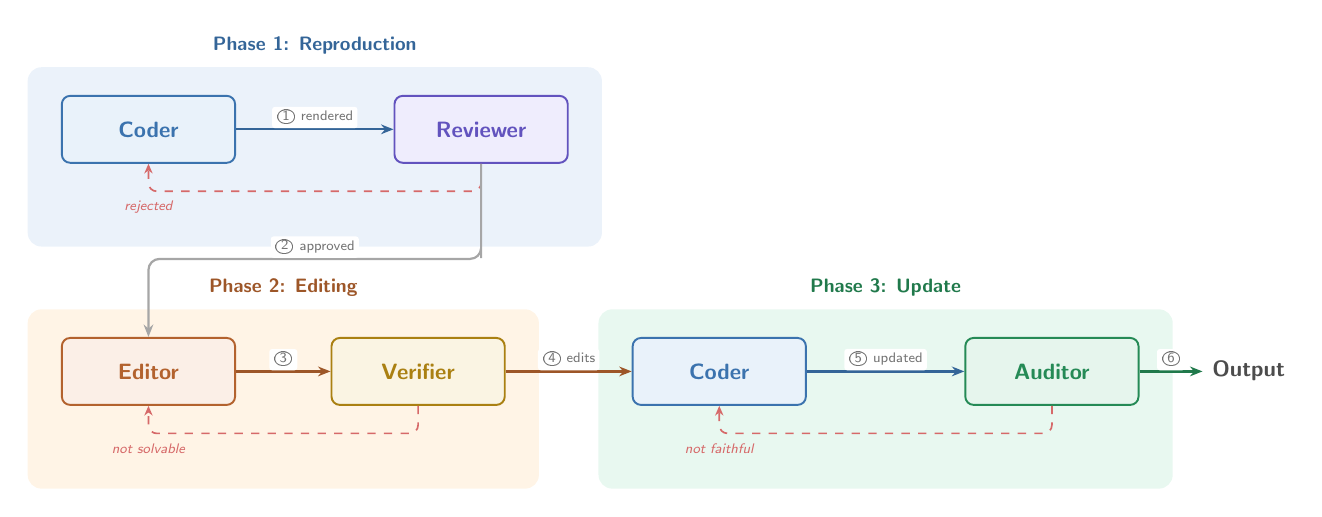
\begin{tikzpicture}

% =============================================
% Row 1: Phase 1 (Reproduction)
% =============================================
\node[agent=coder] (coder1) {Coder};
\node[agent=reviewer, right=2.0cm of coder1] (reviewer) {Reviewer};
\coordinate[below=0.7cm of coder1] (loop1anchor);

% =============================================
% Row 2: Phase 2 (Editing) + Phase 3 (Update)
% Editor aligned under Coder1
% =============================================
\node[agent=editor, below=2.2cm of coder1] (editor) {Editor};
\node[agent=verifier, right=1.2cm of editor] (verifier) {Verifier};
\coordinate[below=0.7cm of editor] (loop2anchor);

\node[agent=coder, right=1.6cm of verifier] (coder2) {Coder};
\node[agent=auditor, right=2.0cm of coder2] (auditor) {Auditor};
\coordinate[below=0.7cm of coder2] (loop3anchor);

\node[right=0.8cm of auditor, font=\sffamily\footnotesize\bfseries, text=black!70] (output) {Output};

% =============================================
% Background boxes — aligned edges
% =============================================
\begin{scope}[on background layer]
    % Phase 2 and Phase 3: natural fit
    \node[fit=(editor)(verifier)(loop2anchor),
          fill=phasebg2, rounded corners=5pt,
          inner xsep=12pt, inner ysep=10pt] (phase2bg) {};
    \node[fit=(coder2)(auditor)(loop3anchor),
          fill=phasebg3, rounded corners=5pt,
          inner xsep=12pt, inner ysep=10pt] (phase3bg) {};

    % Phase 1: natural fit, same inner padding as Phase 2 and Phase 3
    \node[fit=(coder1)(reviewer)(loop1anchor),
          fill=phasebg1, rounded corners=5pt,
          inner xsep=12pt, inner ysep=10pt] (phase1bg) {};
\end{scope}

\node[phaselabel=coder, above=1pt of phase1bg.north] {Phase 1: Reproduction};
\node[phaselabel=editor, above=1pt of phase2bg.north] {Phase 2: Editing};
\node[phaselabel=auditor, above=1pt of phase3bg.north] {Phase 3: Update};

% =============================================
% Phase 1 arrows
% =============================================
\draw[flow=coder] (coder1) -- node[steplabel, above] {\textcircled{\tiny 1}~rendered} (reviewer);

\draw[loopback, rounded corners=3pt]
    (reviewer.south) -- ++(0, -0.35)
    -| node[looplabel, pos=0.5, below] {rejected}
    (coder1.south);

% =============================================
% Phase 2 arrows
% =============================================
\draw[flow=editor] (editor) -- node[steplabel, above] {\textcircled{\tiny 3}} (verifier);

\draw[loopback, rounded corners=3pt]
    (verifier.south) -- ++(0, -0.35)
    -| node[looplabel, pos=0.5, below] {not solvable}
    (editor.south);

% =============================================
% Phase 3 arrows
% =============================================
\draw[flow=editor] (verifier) -- node[steplabel, above] {\textcircled{\tiny 4}~edits} (coder2);
\draw[flow=coder] (coder2) -- node[steplabel, above] {\textcircled{\tiny 5}~updated} (auditor);
\draw[flow=auditor] (auditor) -- node[steplabel, above] {\textcircled{\tiny 6}} (output);

\draw[loopback, rounded corners=3pt]
    (auditor.south) -- ++(0, -0.35)
    -| node[looplabel, pos=0.5, below] {not faithful}
    (coder2.south);

% =============================================
% Cross-row connector: Reviewer -> Editor
% =============================================
\draw[connector, rounded corners=4pt]
    (reviewer.south) -- (reviewer.south |- phase1bg.south)
    -- ++(0, -0.15)
    -| node[steplabel, pos=0.25, above] {\textcircled{\tiny 2}~approved}
    (editor.north);

\end{tikzpicture}
\end{document}
